\documentclass[8pt]{beamer}

\usepackage[T1]{fontenc}		% Selecao de codigos de fonte.
\usepackage[utf8]{inputenc}

\usepackage{lmodern}			% Usa a fonte Latin Modern
\usepackage{amsmath}
\usepackage{amsfonts}
\usepackage{amssymb}
\usepackage{bm}
\usepackage{pgfplots} % graficos
\usepackage{algpseudocode}
\usepackage{algorithm}
\usepackage{multirow}
\usepackage{subcaption}
\usepackage{arydshln}
\usepackage{ulem}
\ULforem

\newcommand{\dtree}[1]{$#1$-d~tree}
\newcommand{\kdtree}{\dtree{k}}
\newcommand{\bsym}[1]{\boldsymbol{#1}}
%\newcommand{\sol}[1]{\boldsymbol{#1}}
\newcommand{\sol}[1]{#1}
\newcommand{\pnt}[1]{pnt(\sol{#1})}
\newcommand{\fsol}[1]{f(\sol{#1})}
\newcommand{\np}{m}
\newcommand{\nphard}{$\mathcal{NP}$-Hard}
\newcommand{\missingI}[1]{}
\newcommand{\missing}[1]{
  \begin{framed}
    {\scriptsize  #1}
  \end{framed}
}
\newcommand{\weight}[1]{w(\sol{#1})}
\newcommand{\obj}[2]{f_{#1}(\sol{#2})}
\newcommand{\bigweight}[1]{w\big(\sol{#1}\big)}
\newcommand{\dom}[2]{dom(\sol{#1}, \sol{#2})}
\newcommand{\domk}[2]{dom_k(\sol{#1}, \sol{#2})}
\newcommand{\setIN}{\{1, \ldots, n\}}
\newcommand{\ext}[2]{ext(\sol{#1}, \sol{#2})}
\newcommand{\domLess}[2]{ \sol{#1} \prec \sol{#2} }
%\newcommand{\logicAnd}{ \textrm{ and } }
\newcommand{\logicAnd}{ \land }
\newcommand{\logicOr}{ \lor}
\newcommand{\solSetA}{ Q }
\newcommand{\solSetB}{ R }
\newcommand{\solSett}{ S_* }
\newcommand{\solSet}{ S }
\newcommand{\rord}{\mathcal{O}_{rev}}
\newcommand{\cb}[2]{cb^{#1}(#2)}  % cost-benefit function
\renewcommand{\leq}{\leqslant}
\renewcommand{\geq}{\geqslant}
\newcommand{\floor}[1]{\left \lfloor{#1}\right \rfloor}

% bar graphs configs
\newcommand{\cmpH}{4.0cm}
\newcommand{\cmpW}{7cm}
\newcommand{\legX}{0.45}
\newcommand{\legY}{-0.30}
\newcommand{\scecore}{SCEcr }
\newcommand{\mokp}{MOKP}
\newcommand{\paretoset}{conjunto Pareto}
\newcommand{\paretosetII}{conjunto Pareto-ótimo}
\newcommand{\knapsackdominates}{domina segundo a mochila}

% big bullet
\newcommand{\bbt}{\,\begin{picture}(-1,1)(-1,-2)\circle*{5}\end{picture}\ }

\newcommand{\ord}{\mathcal{O}}
\newcommand{\fvar}[1]{}

% bullet do itemize
\setbeamertemplate{itemize items}[circle]
% estilo do título
\setbeamertemplate{frametitle}{\bigskip \color{black}\bfseries\insertframetitle}

\title{A Hybrid Heuristic for the Multi-objective Knapsack Problem}
\subtitle{Doctoral thesis proposal}
\author{Marcos Daniel V. Baroni}
\institute[UFES - DI - PPGI]{
  Universidade Federal do Espírito Santo \\
  Departamento de Informática \\
  Programa de Pós-graduação em Informática}
\date{27 de novembro de 2017}

\usetheme{Szeged}
\usecolortheme{seahorse}

\begin{document}

% Title Page
\frame{\titlepage}

% Sumário
\begin{frame}
\frametitle{Table of Contents}
\tableofcontents
\end{frame}

% Introdução
\section{A Hybrid Heuristic for the Multi-objective Knapsack Problem}
\subsection{Introduction}
%  - The problem and its application
%  - Literature background
%  - The Bazgan algorithm
%  - Our approach (motivation and use of KDTRee)
%  - Article structure


% Introdução
%\section{A Hybrid Heuristic for the Multi-objective Knapsack Problem}
\subsection{The Multi-objective Knapsack Problem}
% Breve definicao de multiobjective opt
A general multiobjective optimization problem can be described as a vector
function $f$ that maps a tuple of $n$ parameters (decision variables) to a tuple
of $\np$ objectives.
Formally:
\begin{align*}
  \text{min/max} ~ \sol{y} &= f(\sol{x}) = 
    \big(f_1(\sol{x})
    ,f_2(\sol{x})
    ,\ldots
    ,f_{\np}(\sol{x})\big) \\
  \text{subject to} ~ \sol{x} & = (x_1, x_2, \ldots, x_n) \in X
\end{align*}
where $\sol{x}$ is called the \emph{decision vector} or \emph{solution}, $X$ denotes the set
of feasible solutions, and $\sol{y}$ is the \emph{objective vector} or \emph{criterion vector} where
each objective has to be minimized (or maximized).

Considering two decision vectors $\sol{a}, \sol{b} \in X$, $a$ is said to
\emph{dominate} $b$ if, and only if:
\begin{align*}
    \forall i &\in \{1, 2, \ldots, \np\}: f_i(\sol{a}) \geq f_i(\sol{b}) \\
    \exists j &\in \{1, 2, \ldots, \np\}: f_j(\sol{a}) > f_j(\sol{b})
\end{align*}

A solution $\sol{a} \in X$ is called \emph{efficient} or \emph{non-dominated}
if there is not other feasible solution $\sol{b} \in X$ such that $\sol{b}$ dominates $\sol{a}$.
The set of solutions of a multiobjective optimization problem consists of all efficient solutions.
This set is known as \emph{Pareto optimal}.

The instance of a multiobjective knapsack problem with $\np$
objectives consists of an integer capacity $W > 0$ and $n$ items.
Each item $i$ has a positive weight $w^i$ and $\np$ non negative integer
profits $p_{i}^{1}, \ldots, p_{i}^{\np}$.
A solution is represented by a vector $\sol{x} = (x_1, \ldots, x_n)$ of binary
decision variables $x_i$, such that $x_i = 1$ if item $i$ is included in the
solution and $0$ otherwise, satisfing the capacity of the knapsack.
For any instance of the problem, we aim at determining the set of efficient solutions.

Formally the definition of the problem is:
\begin{align*}
    \text{max   } & f(\sol{x}) = 
      \big(f_1(\sol{x}) ,f_2(\sol{x}) ,\ldots ,f_{\np}(\sol{x})\big) \\
    \text{subject to   } & w(\sol{x}) < W \\
    & x_{i} \in \{0, 1\} \quad i = 1, \ldots, n \\
    \text{where} \phantom{mmmmm} \\
    f_j(\sol{x}) &= \sum_{i=1}^{n} v^j_i x_i \quad j = 1, \ldots, \np \\
    w(\sol{x}) &= \sum_{i=1}^{n} w_i x_i
\end{align*}

The MOKP is considered a \nphard{} problem, since it is a generalization
of the well-known 0$-$1 knapsack problem and
it is quite difficult to determine the Pareto optimal set for the MOKP,
especially for high dimension instances, in which the Pareto set it self tends
to grow exponentially.
For this reason, the development of methods efficiently deal with high-dimension
instances is...

% Definições, Propriedados e teoremas para o MOKP: dominancia



%\section{A Hybrid Heuristic for the Multi-objective Knapsack Problem}
\subsection{The Multi-dimensional Indexing}
% Falar sobre a utilização de estrutura de dados.

\section{Verificação de dominância e a busca de faixa}

Como dito anteriormente, solucionar um problema multi-objetivo significa
apresentar o seu \paretoset{}, ou seja, o conjunto de soluções não dominadas.
Geralmente o processo de solução compreende-se em contruir este conjunto de
soluções de forma incremental.
Por este motivo, um dos procedimentos mais executados durante o processo é
verificar se uma determinada solução é dominada por alguma outra solução
existente num conjunto candidato.
Um algoritmo pode até mesmo necessitar de extrair um cojunto cobertura, ou seja,
extrair todas as soluções não-dominadas de um grande conjuto de soluções.

Esta operação deve demandar exforço quadrático sobre o número total de soluções
se implementada como uma comparação par-a-par.
Entretanto, se as soluções forem interpretadas como pontos em um espaço
multi-dimensional, podemos deduzir da Equação~\ref{eq:dom} que esta operação
corresponde em verificar a existência um ponto numa determinada região
do espaço. O mesmo pode ser considerado no caso mais específico para a dominância
da mochila, segundo a Equação~???.
Formalmente:
\begin{align*}
    & x \dom y \; \Longleftrightarrow \; \pnt{y} \in R(\sol{x}) \\
  \text{where} \phantom{mmmmm} \\
    \pnt{x} &= \big(\obj{1}{x}, \ldots, \obj{\np}{x}, \weight{x}\big) \\
    R(\sol{x}) &= \left\{ a \in \mathbb{R}^{\np+1} \;\middle|\;
      a_{\np+1} \leq \weight{x}
      \, \text{ and } \,
      a_i \geq \obj{i}{x}, \; i \in \{1, \ldots, \np\}
      \right\}
\end{align*}

\missing{Colocar referência para a equação de dominância da mochila (texto acima).}

O problema de determinar a existência de um ponto numa determinada região do
espaço é já bem conhecido da computação e chama-se problema da
\emph{busca de baixa} (ou \emph{range search} em ingês)~\cite{agarwal1999geometric}.
O problema de busca de faixa é largamente aplicado, por exemplo, na área da
computação gráfica e jogos, onde é necessário se verificar a colisão entre pontos e polígonos.
Para se ter uma solução eficiente deste problema evitando o esforço computacional
quadrático, os pontos devem ser indexados multidimensional.....
\missing{Melhorar parágrafo acima e conferir texto inicial do parágrafo abaixo.}

Devido a sua simplicidade e eficiência, a estrutura de dados mais utilizada
para o problema é a \emph{\kdtree}~\cite{preparata2012computational}.
Proposta por Jon Louis Bentley em 1957~\cite{bentley1975}, a \kdtree{} é um tipo de
árvore binária de construção simples e baixa utilização de memória.
Apesar de sua simplicidade, além da operação de buca de faixa, a \kdtree{}
suporta outras operações como busca de vizinho mais próximo.
Por este motivo é também bastante utilizada em algoritmos de
clasterização~\cite{kanungo2002efficient, indyk1998approximate}
e renderização gráfica~\cite{owens2007survey}.

Como uma árvore binária comum, a cada nível recursivo da árvore
a \kdtree{} subdivide os dados em duas partes.
Porém, diferentemente de uma árvore de busca binária comum, as quais utilizam
apenas uma \emph{chave} em todos os níveis da árvore, a \kdtree{} utiliza um
total de $k$ chaves fazendo um revezamento circular entre as chaves à medida
que caminha nos níveis da árvore.

A Figura~\ref{fig:kdom-kd} apresenta (a) um conjunto de pontos dispostos num
espaço bi-dimensional e indexados por uma (b) \dtree{2}.
O primeiro e terceiro nível da \dtree{2} indexa a componente $x$ dos pontos,
enquanto o segundo nível indexa a componente $y$.
Cada ponto indexado pela árvore subdivide o espaço em dois de acordo
com o valor da componente que está sendo indexada.
A subdivisão do espaço é representada na figura por uma linha mais grossa.

\begin{figure}[H]
  \centering
  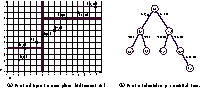
\includegraphics[scale=4.8]{img/kdt/dom-kd}
  \caption{Exemplo de pontos indexados por uma \kdtree{}.}
  \label{fig:kdom-kd}
\end{figure}

A Figura~\ref{fig:query} apresenta um exemplo de operação de verificação de
dominância utilizando uma \dtree{2} como estrutura de indexação.
A área acinzentada não tem intersecção com a área dominada pelo ponto $x$
(área hachurada), portanto as soluções dentro da área acinzentada não são
avaliadas.

\missing{Propor passo-a-passo da operação.}

\begin{figure}[H]
  \centering
  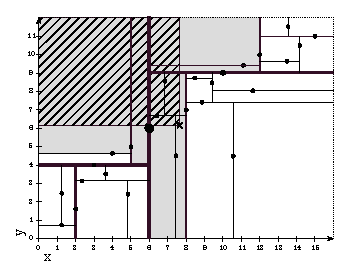
\includegraphics[scale=1.7]{img/kdt/query}
  \caption{Exemplo de operação de verificação de dominância utilizando a \kdtree{}.}
  \label{fig:query}
\end{figure}

Com relação à eficiência da \kdtree{} é importante considerar que não é
recomendável escalar de forma arbitrária o número $k$ de dimensões
indexadas pela \kdtree{}, esperando assim escalar também sua eficiência.
Mesmo que o dado possua todas estas dimensões.
Como regra geral considera-se que um \kdtree{} é adequada para indexar um
conjunto com $n$ pontos se $n$ não for muito maior que $2^k$\cite{toth2004handbook},
caso contrário, a performance da \kdtree{} se assemelhará a de uma busca
linear exaustiva.

Espera-se que a \kdtree{} auxilie as operações de verificação de dominância
\emph{podando} uma grande quantidade de soluções, demandando um menor número
de comparações entre soluções, melhorando assim a performance dos algoritmos.

% Falar um pouco sobre arvore binária.

% Definir a árvore kdtree


%\section{A Hybrid Heuristic for the Multi-objective Knapsack Problem}
\subsection{The Shuffled Complex Evolution}

%
\begin{frame}
\frametitle{}
\begin{center}
  \textbf{\Large The Shuffled Complex Evolution}
\end{center}
\end{frame}

%
\begin{frame}
\frametitle{The Shuffled Complex Evolution}
\begin{columns}
\begin{column}{0.75\textwidth}  %%<--- here
  {\small
  The SCE  regards a natural  evolution happening
  simultaneously in independent communities;
  \\ \medskip \pause
  A population of $N*M$ individuals is randomly taken from the
  solution space;
  \\ \medskip \pause
  The population is then sorted by descending order of fitness
  and the best global solution is identified;
  \\ \medskip \pause
  The population is then shuffled into $N$ complexes,
  each containing $M$ individuals;
  \\ \medskip \pause
  In this shuffling process the first individual goes to the first complex, the second
  individual goes to the second complex, individual $N$ goes to $N$-th complex,
  individual $(M+1)$-th goes back to the first complex, etc;
  \\ \medskip \pause
  The next step after shuffling the complexes is to evolve each complex.
  }
\end{column} \pause
\begin{column}{0.25\textwidth}
  \hspace{-15pt}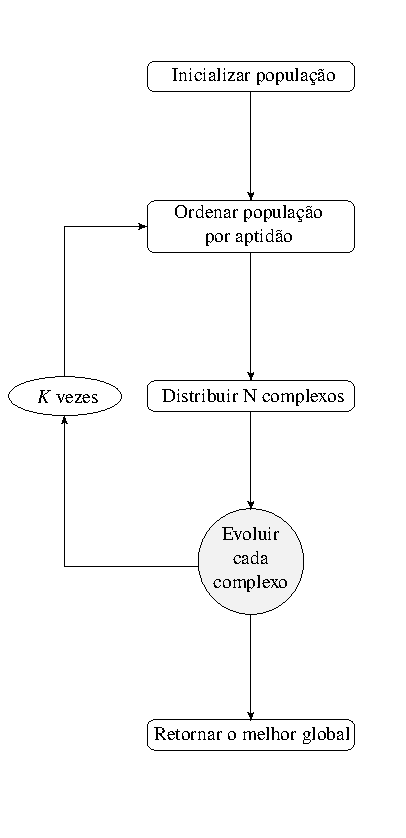
\includegraphics[scale=0.45]{img/sce/flow1}
\end{column}
\end{columns}
\end{frame}

%
\begin{frame}
\frametitle{The Shuffled Complex Evolution}
\begin{columns}
\begin{column}{0.75\textwidth}  %%<--- here
  {\small
  In each step a subcomplex of $P$ individuals is selected from the
  complex;
  \\ \medskip \pause
  After the selection of the subcomplex, its worst individual is identified to
  be replaced by a new generated solution;
  \\ \medskip \pause
  This new solution is generated by the crossing of the worst individual and an
  other individual with better fitness;
  \\ \medskip \pause
  At first the best individual of the subcomplex is considered for the crossing;
  \\ \medskip \pause
  If the new solution is not better than the worst one, the best individual
  of the complex is considered for a crossing;
  \\ \medskip \pause
  If the latter crossing did not result in any improvement, the best individual
  of whole population is considered;
  \\ \medskip \pause
  Finally, if all the crossing steps couldn't generate a better individual,
  the worst individual of the subcomplex is replaced by a new random solution taken
  from the feasible solution space.
  }
\end{column} \pause
\begin{column}{0.25\textwidth}
  \vspace{10pt}\hspace{-18pt}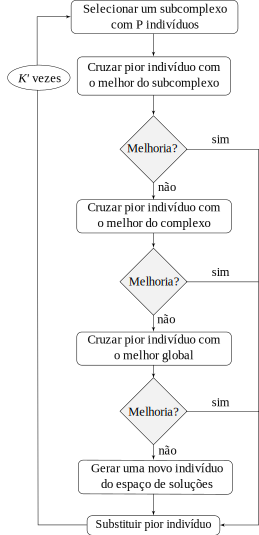
\includegraphics[scale=0.45]{img/sce/flow2}
\end{column}
\end{columns}
\end{frame}

%
\begin{frame}
\frametitle{}
\begin{center}
  \textbf{\Large The Shuffled Complex Evolution}
  \\ \bigskip \bigskip
  {\large Use case for the MKP}
\end{center}
\end{frame}

% The SCE for MKP
\begin{frame}
\frametitle{The SCE for MKP}
the SCE is easily applied to any
optimization problem.
The only steps needed to be specified is \textbf{(a)} the creation of a new random
solution and \textbf{(b)} the crossing procedure of two solutions.
\end{frame}

% Random for MKP
\begin{frame}
\frametitle{The SCE for MKP}
New random solution generation for the MKP.
\begin{figure}
\begin{algorithmic}[1]
  \Function{New random solution}{} \pause
    \State $v \leftarrow $ shuffle($1, 2, \ldots, n$) \pause
	\State $s \leftarrow \emptyset$ \pause
    \For{$ i \leftarrow 1:n$ }
	  \State $s \leftarrow s \cup \{v_i\}$ \pause
	  \If{ $s$ is not feasible} \pause
	    \State $s \leftarrow s - \{v_i\}$
      \EndIf  \pause
	\EndFor
  \State return $s$
  \EndFunction
\end{algorithmic}
\end{figure}
\end{frame}

% Crossing for MKP
\begin{frame}
\frametitle{The SCE for MKP}
Crossing procedure for the MKP.
\begin{figure}
\begin{algorithmic}[1]
  \Function{Crossing}{$x^w:$ worst individual, $x^b:$ better individual, $c$} \pause
    \State $v \leftarrow $ shuffle($1, 2, \ldots, n$) \pause
    \For{$ i \leftarrow 1:c$ }
	  \State $j \leftarrow v_i$ \pause
	  \State $x^w_j \leftarrow x^b_j$
	\EndFor \pause
	\If{$s^w$ is not feasible}
	  \State repair $s^w$
	\EndIf \pause
  \State return $s^w$
  \EndFunction
\end{algorithmic}
\end{figure}
\end{frame}


% SCE parameters
\begin{frame}
\frametitle{Computational Experiments}
Parameters used for SCE:
\begin{itemize}
  \item $N = 20$: number of complexes;
  \item $M = 20$: number of individuals in each complex;
  \item $P = 5$: number of individuals in each subcomplex;
  \item $K = 300$: number of algorithm iterations;
  \item $K' = 20$: number of iterations used in the complex evolving process;
  \item $c = n/5$: number of genes carried from parent in crossing process.
\end{itemize}
\end{frame}

% Results (chub)
\begin{frame}
\frametitle{Computational Experiments}
SCE and \scecore  performance on Chu-Beasley problems.
\begin{table}[hb]
{
\renewcommand{\arraystretch}{0.7}%
\fontsize{4.5pt}{1em}\selectfont
\begin{center}
  \begin{tabular}{|r|r|r|rr|rr|} \cline{4-7}
  \multicolumn{3}{c|}{} &
    \multicolumn{2}{c|}{\bf time (s)} &
    \multicolumn{2}{c|}{\bf quality (\%)} \\ \hline
  \textbf{n}   &
    \textbf{m}  &
    \textbf{$\alpha$} &
    \textbf{SCE} &
    \textbf{\scecore} &
    {\bf SCE} &
    {\bf \scecore}  \\ \hline
{\bf  100}   &  {\bf 5} & 0.25 & 1.22\fvar{0.04} & 0.17\fvar{0.00} & 96.51\fvar{0.92} & 99.73\fvar{0.04} \\
        &    & 0.50 & 1.34\fvar{0.02} & 0.18\fvar{0.00} & 97.42\fvar{0.55} & 99.86\fvar{0.01} \\
        &    & 0.75 & 1.37\fvar{0.03} & 0.17\fvar{0.00} & 98.87\fvar{0.20} & 99.91\fvar{0.00} \\ \cline{2-7}
        & {\bf 10} & 0.25 & 1.32\fvar{0.04} & 0.25\fvar{0.00} & 95.68\fvar{1.28} & 99.53\fvar{0.09} \\
        &    & 0.50 & 1.51\fvar{0.04} & 0.25\fvar{0.00} & 96.65\fvar{0.49} & 99.76\fvar{0.03} \\
        &    & 0.75 & 1.46\fvar{0.04} & 0.27\fvar{0.00} & 98.54\fvar{0.19} & 99.96\fvar{0.00} \\ \cline{2-7}
        & {\bf 30} & 0.25 & 1.74\fvar{0.06} & 1.20\fvar{0.03} & 95.38\fvar{1.01} & 97.96\fvar{0.22} \\
        &    & 0.50 & 1.79\fvar{0.08} & 0.89\fvar{0.06} & 96.41\fvar{0.63} & 99.18\fvar{0.06} \\
        &    & 0.75 & 1.72\fvar{0.09} & 0.95\fvar{0.04} & 98.18\fvar{0.33} & 99.52\fvar{0.04} \\ \hline
{\bf  250} & {\bf 5} & 0.25 & 2.87\fvar{0.07} & 0.69\fvar{0.01} & 93.22\fvar{0.64} & 99.86\fvar{0.00} \\
        &    & 0.50 & 2.82\fvar{0.11} & 0.70\fvar{0.01} & 94.88\fvar{0.21} & 99.94\fvar{0.00} \\
        &    & 0.75 & 2.93\fvar{0.08} & 0.69\fvar{0.01} & 97.57\fvar{0.10} & 99.96\fvar{0.00} \\ \cline{2-7}
        & {\bf 10} & 0.25 & 3.08\fvar{0.09} & 0.87\fvar{0.01} & 93.14\fvar{0.67} & 99.58\fvar{0.01} \\
        &    & 0.50 & 3.03\fvar{0.09} & 0.79\fvar{0.02} & 94.55\fvar{0.26} & 99.79\fvar{0.00} \\
        &    & 0.75 & 3.12\fvar{0.09} & 0.84\fvar{0.01} & 97.16\fvar{0.13} & 99.88\fvar{0.00} \\ \cline{2-7}
        & {\bf 30} & 0.25 & 3.74\fvar{0.12} & 1.52\fvar{0.04} & 93.10\fvar{0.74} & 98.42\fvar{0.08} \\
        &    & 0.50 & 3.74\fvar{0.16} & 1.36\fvar{0.06} & 94.20\fvar{0.30} & 99.33\fvar{0.02} \\
        &    & 0.75 & 3.99\fvar{0.13} & 1.48\fvar{0.04} & 96.64\fvar{0.14} & 99.59\fvar{0.01} \\ \hline
{\bf  500} & {\bf 5} & 0.25 & 5.62\fvar{0.10} & 1.25\fvar{0.02} & 91.37\fvar{0.50} & 99.77\fvar{0.00} \\
        &    & 0.50 & 5.72\fvar{0.19} & 1.24\fvar{0.01} & 93.39\fvar{0.27} & 99.88\fvar{0.00} \\
        &    & 0.75 & 5.88\fvar{0.14} & 1.20\fvar{0.02} & 96.42\fvar{0.06} & 99.92\fvar{0.00} \\ \cline{2-7}
        & {\bf 10} & 0.25 & 5.97\fvar{0.17} & 1.41\fvar{0.02} & 91.62\fvar{0.50} & 99.51\fvar{0.01} \\
        &    & 0.50 & 6.11\fvar{0.23} & 1.36\fvar{0.03} & 93.09\fvar{0.20} & 99.77\fvar{0.00} \\
        &    & 0.75 & 5.47\fvar{0.61} & 1.21\fvar{0.03} & 96.24\fvar{0.06} & 99.84\fvar{0.00} \\ \cline{2-7}
        & {\bf 30} & 0.25 & 6.20\fvar{1.14} & 1.96\fvar{0.22} & 91.37\fvar{0.82} & 98.76\fvar{0.02} \\
        &    & 0.50 & 6.26\fvar{1.07} & 1.82\fvar{0.14} & 92.56\fvar{0.13} & 99.42\fvar{0.01} \\
        &    & 0.75 & 6.05\fvar{1.16} & 1.73\fvar{0.20} & 95.97\fvar{0.06} & 99.67\fvar{0.00} \\ \hline
\end{tabular}

\end{center}
}
\end{table}
\end{frame}

% Results (gk)
\begin{frame}
\frametitle{Computational Experiments}
\scecore performance on Glover-Kochenberger problems.
\begin{table}[hb]
  {
  \renewcommand{\arraystretch}{1}%
  \fontsize{5.5pt}{1em}\selectfont
  \begin{center}
    \begin{tabular}{|r|r|r|c|r|r|r|} \cline{4-7}
  \multicolumn{3}{c|}{} &
    \multicolumn{2}{c|}{\bf time (s)} &
    \multicolumn{2}{c|}{\bf quality (\%)} \\ \hline
  \textbf{\#} &
    \textbf{n}   &
    \textbf{m}  &
    {\bf SCE } &
    {\bf SCEcr } &
    {\bf SCE} &
    {\bf SCEcr} \\ \hline
  01   &  100 &  15 &   1.47\fvar{0.00} & 0.08\fvar{0.0} & 97.66\fvar{0.03} & 99.24\fvar{0.02} \\ \hline
    02 &  100 &  25 &   1.61\fvar{0.00} & 0.09\fvar{0.0} & 97.94\fvar{0.04} & 98.94\fvar{0.09} \\ \hline
    03 &  150 &  25 &   2.51\fvar{0.01} & 0.09\fvar{0.0} & 97.22\fvar{0.04} & 99.09\fvar{0.02} \\ \hline
    04 &  150 &  50 &   3.56\fvar{0.03} & 0.09\fvar{0.0} & 97.40\fvar{0.04} & 98.52\fvar{0.02} \\ \hline
    05 &  200 &  25 &   3.55\fvar{0.01} & 0.09\fvar{0.0} & 96.88\fvar{0.03} & 99.28\fvar{0.01} \\ \hline
    06 &  200 &  50 &   4.81\fvar{0.09} & 0.10\fvar{0.0} & 97.68\fvar{0.02} & 98.90\fvar{0.03} \\ \hline
    07 &  500 &  25 &   7.30\fvar{0.09} & 0.10\fvar{0.0} & 97.12\fvar{0.01} & 99.54\fvar{0.00} \\ \hline
    08 &  500 &  50 &  12.20\fvar{0.47} & 0.11\fvar{0.0} & 97.27\fvar{0.01} & 99.33\fvar{0.01} \\ \hline
    09 & 1500 &  25 &  24.61\fvar{1.73} & 0.12\fvar{0.0} & 95.40\fvar{0.01} & 98.22\fvar{0.00} \\ \hline
    10 & 1500 &  50 &  33.79\fvar{2.44} & 0.13\fvar{0.0} & 97.50\fvar{0.00} & 99.64\fvar{0.00} \\ \hline
    11 & 2500 & 100 & 121.28\fvar{194.74} & 0.15\fvar{0.0} & 97.95\fvar{0.00} & 99.70\fvar{0.00} \\ \hline
\end{tabular}

  \end{center}
  }
\end{table}
\end{frame}

% Results (gk)
\begin{frame}
\frametitle{Conclusions}
The SCE algorithm for MKP proved to be able to achieve fast
convergence ratio, finding good quality near optimal solutions, demanding small
amount of computational time.
\\ \medskip \pause
The core concept as a variable fixing procedure
proved to be efficient to reduce the size of the problems which provided fast
execution time, producing higher quality solutions.
\\ \medskip \pause
At least $99.02\%$ of best known, in less than $2$ seconds for every instance.
\end{frame}


%\section{A Hybrid Heuristic for the Multi-objective Knapsack Problem}
\subsection{The Shuffled Complex Evolution}
%
\begin{frame}
\frametitle{}
\begin{center}
  \textbf{\Large A SCE for the MOKP}
\end{center}
\end{frame}

%
\begin{frame}
\frametitle{A SCE for the MOKP}
As seen in previous sections
the SCE is easily applied to any optimization problem.
\\ \bigskip \pause
The fact that the MKP shares the same solution representation
as the MOKP allow us to use the same procedures
used on MKP.
\end{frame}

%
\begin{frame}
\frametitle{Non-dominated Sort}
Fitness computation for multi-objective solutions.
\medskip
\begin{columns}
\begin{column}{0.5\textwidth}  %%<--- here
  \begin{algorithmic}[1]
    \Function{NDSort}{$S:$ solution set}
      \State $i = 0$
      \While{ $S \neq \emptyset$ }
        \For{ $\sol{s} \in S$}
          %\State $D = \{ x \in X | \dom{x}{s}\}$
          \If{ $\nexists \sol{x} \in S : \dom{x}{s}$ }
            \State $o_s = i$
            \State $S = S - {x}$
          \EndIf
        \EndFor
        \State $i = i+1$
      \EndWhile
    \EndFunction
  \end{algorithmic}
\end{column}
\begin{column}{0.5\textwidth}
  \begin{figure}
    \centering
    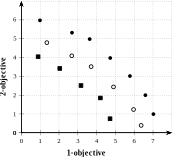
\includegraphics{img/pareto-sort}
  \end{figure}
\end{column}
\end{columns}
\end{frame}


%
\begin{frame}
\frametitle{Non-dominated Sort}
Fitness computation for multi-objective solutions.
\medskip

\end{frame}


% Schedule
\begin{frame}
\frametitle{Preliminary Computational Experiments}
Time and quality for bi-dimensional instances:
\begin{table}
\centering
{
\begin{tabular}{|cc|c|cc|}
 \hline
 { \bf Type}
 & {\bf n}
 & {\bf time (s) }
 & {\bf time (s)}
 & { \bf Hypervolume } \\ \hline
 A
 & 120
 & 479.5
 &  46.5
 &  97.0 \% \\ \hline
 B
 & 500
 & 503.6
 &  98.3
 &  98.6 \% \\ \hline
 C
 & 80
 & 559.1
 & 16.2
 & 94.4 \% \\ \hline
 D
 & 40
 & 462.0
 & 92.4
 & 97.2 \% \\ \hline
\end{tabular}
}
\end{table}
\end{frame}

\begin{frame}
\frametitle{Final Doctoral Schedule}
\begin{table}
\centering
{
\def\arraystretch{1.0}%
\fontsize{6.5pt}{1em}\selectfont
\begin{tabular}{|l|c:c:c|c:c:c:c|c:c:c:c|}
 \hline
  \multirow{3}{*}{\textbf{ \phantom{aaaa} Activities}}
  & \multicolumn{11}{c|}{\textbf{Weeks}} \\ \cline{2-12}
   & \multicolumn{3}{c|}{\textbf{ November }}
   & \multicolumn{4}{c|}{\textbf{December}}
   & \multicolumn{4}{c|}{\textbf{January}} \\ \cline{2-12}
  & \;2º\; & 3º & 4º & 1º & 2º & 3º & 4º & 1º & 2º & 3º & 4º \\ \hline
 Literature review
  & $\bbt$ & $\bbt$ & $\bbt$ & & & & & & & & \\ \hline
 Implementation and adjustments
  & $\bbt$ & $\bbt$ & $\bbt$ & $\bbt$ & & & & & & & \\ \hline
 Computational experiments
  & & & $\bbt$ & $\bbt$ & $\bbt$ & & & & & & \\ \hline
 CEC Paper writing
  & & & & & & $\bbt$ & $\bbt$ & $\bbt$ & & & \\ \hline
 CEC Paper submission
  & & & & & & & & & $\bbt$ & & \\ \hline
 Thesis writing
  & & & & $\bbt$ & $\bbt$ & $\bbt$ & $\bbt$ & $\bbt$ & $\bbt$ & $\bbt$ & \\ \hline
\end{tabular}
}
\end{table}
\end{frame}


\end{document}
